\chapter{Ejemplo de ap\'{e}ndice: El problema de la medida}\label{C:ap1}
\chapterquote{Negociemos Don Inodoro}{Fernando de la R\'{u}a, 2001}
\chapterquote{Smartness runs in my family.  When I went to school I was so smart my
teacher was in my class for five years}{George Burns}
\graphicspath{{figs/}}
%%%%%%%%%%%%%%%%%%%%%%%%%%%%%%%%%%%%%%%%%%%%%%%%%%%%%%%%%%%%%%%%%%%%%%%%
El gran problema lo constituye el proceso de medici\'{o}n. En la f\'{\i}sica cl\'{a}sica, medir significa revelar o poner de manifiesto propiedades que estaban en el sistema desde antes de que midamos \cite{Philipp1982NCBSp75}.

En mec\'{a}nica cu\'{a}ntica el proceso de medici\'{o}n altera de forma incontrolada la evoluci\'{o}n del sistema. Constituye un error pensar dentro del marco de la f\'{\i}sica cu\'{a}ntica que medir es revelar propiedades que estaban en el sistema con anterioridad. La informaci\'{o}n que nos proporciona la funci\'{o}n de onda es la distribuci\'{o}n de probabilidades, con la cual se podr\'{a} medir tal valor de tal cantidad. Cuando medimos ponemos en marcha un proceso que es indeterminable a priori, lo que algunos denominan azar, ya que habr\'{a} distintas probabilidades de medir distintos resultados. Esta idea fue y es a\'{u}n objeto de controversias y disputas entre los f\'{\i}sicos, fil\'{o}sofos y epistem\'{o}logos. Uno de los grandes objetores de esta interpretaci\'{o}n fue Albert Einstein, quien a prop\'{o}sito de esta idea dijo su famosa frase "Dios no juega a los dados".

Independientemente de los problemas de interpretaci\'{o}n, la mec\'{a}nica cu\'{a}ntica ha podido explicar esencialmente todo el mundo microsc\'{o}pico y ha hecho predicciones que han sido probadas experimentalmente de forma exitosa, por lo que es una teor\'{\i}a un\'{a}nimemente aceptada.

\begin{figure}[ht]
\centering{}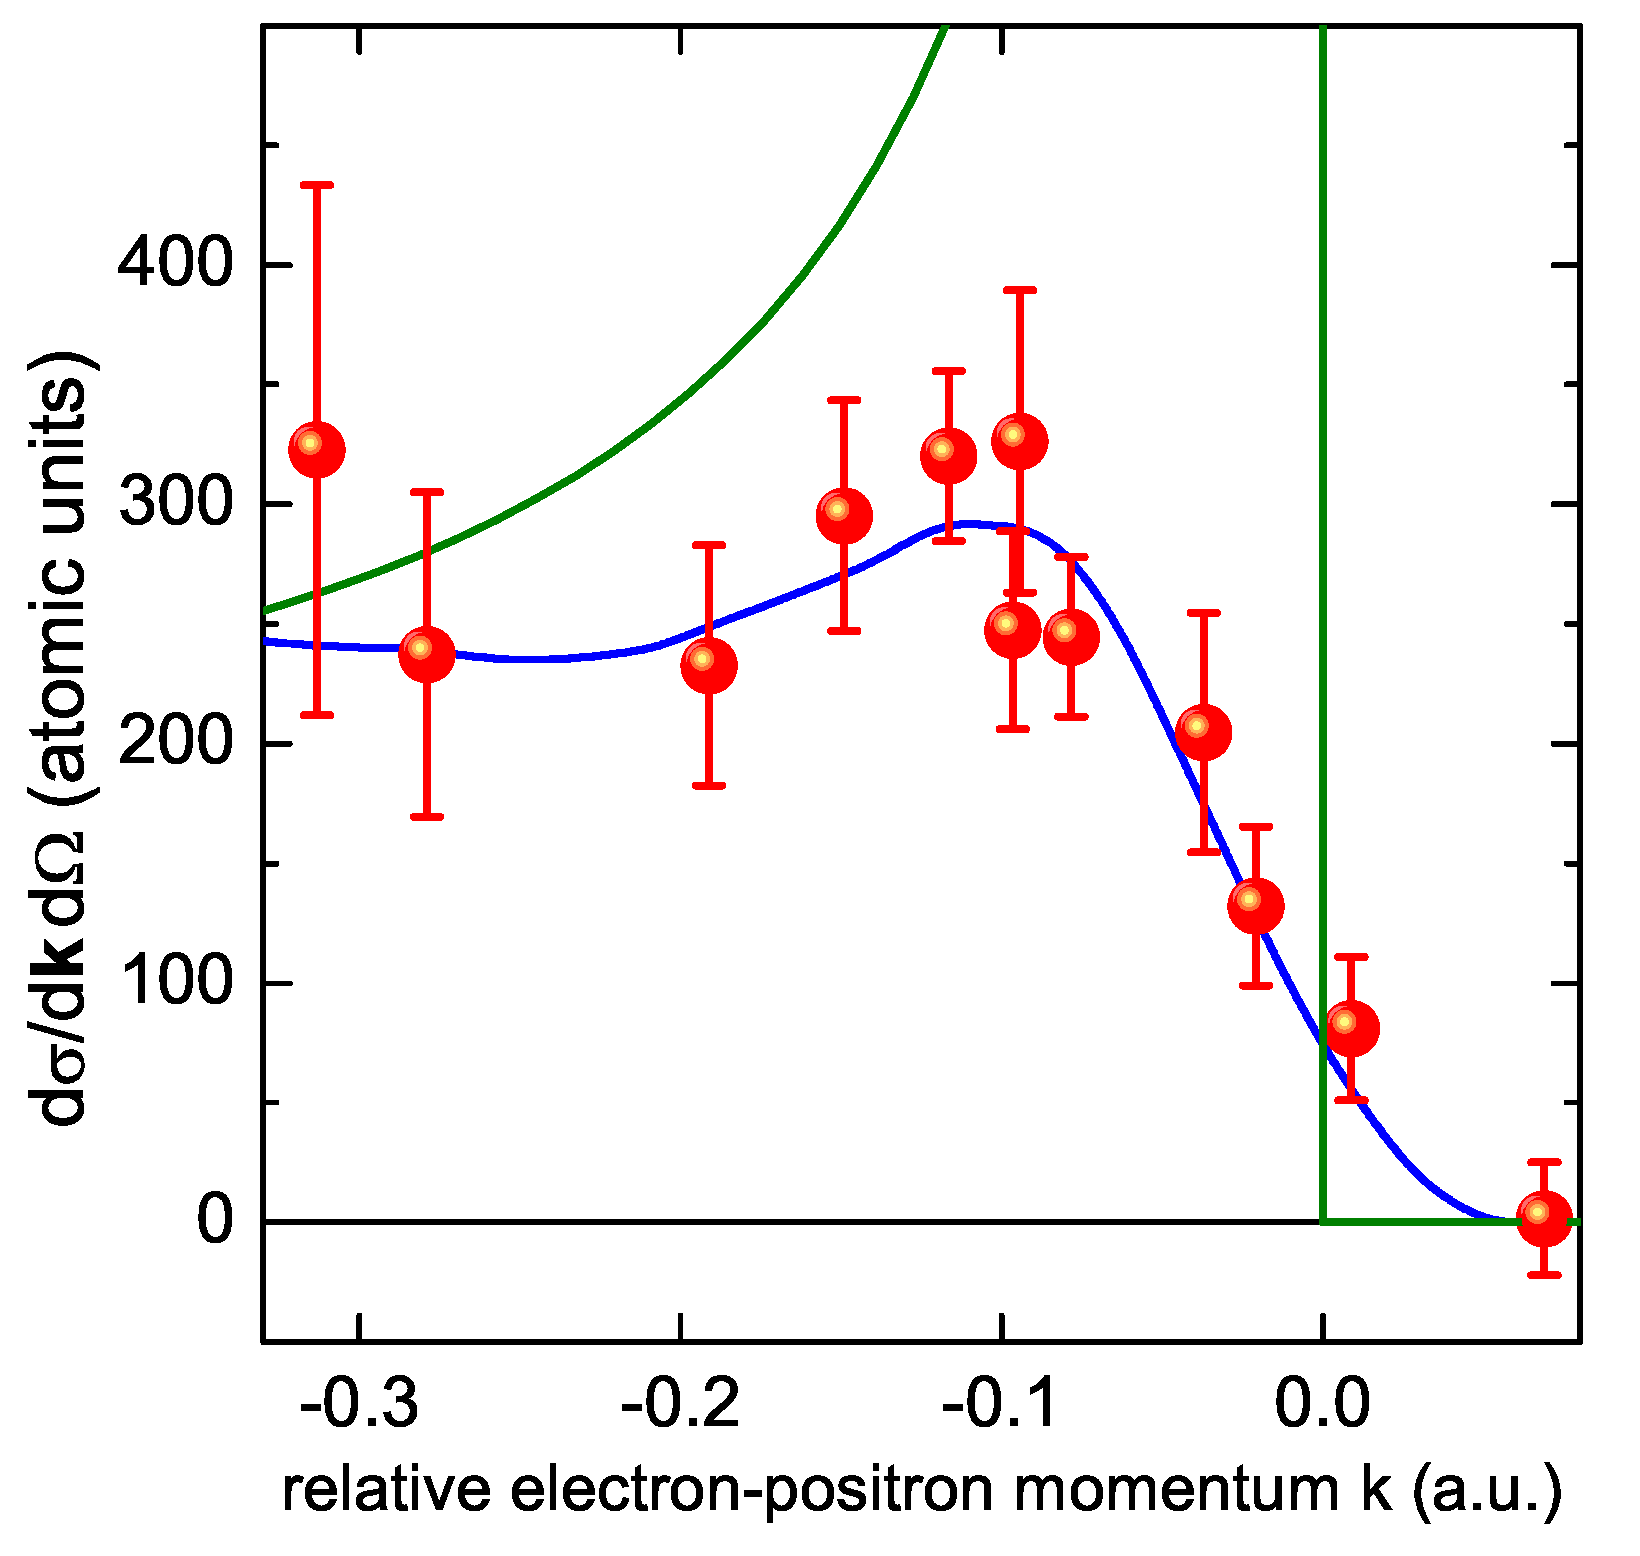
\includegraphics[width=\imsize]{ap1_f1}
\caption{Una figura con algunos puntos experimentales y curva de datos te\'{o}ricos\label{f:figura1}}  
\end{figure}



%%% Local Variables: 
%%% mode: latex
%%% TeX-master: "template"
%%% End: 
